\documentclass{article}

\usepackage{iclr2020_conference,times}

% COMMENT for anonymous submission
% \def\nonanonymous{}

\ifdefined\nonanonymous
\iclrfinalcopy
\fi

% to avoid loading the natbib package, add option nonatbib:
%     \usepackage[nonatbib]{neurips_2019}

\usepackage[utf8]{inputenc} % allow utf-8 input
\usepackage[T1]{fontenc}    % use 8-bit T1 fonts
\usepackage{hyperref}       % hyperlinks
\usepackage{url}            % simple URL typesetting
\usepackage{booktabs}       % professional-quality tables
\usepackage{amsfonts}       % blackboard math symbols
\usepackage{nicefrac}       % compact symbols for 1/2, etc.
\usepackage{microtype}      % microtypography

% Not part of the offical NeurIPS template
\usepackage{amssymb}
\usepackage{amsthm}
\usepackage{bm}
\usepackage{mathtools}
\usepackage{caption}
\usepackage{subcaption}
\usepackage{caption}
\usepackage{csquotes}
\usepackage{layouts}
\usepackage{float}
\usepackage{todonotes}
\usepackage{enumitem}

% Algorithms
\usepackage{algorithm}
\usepackage[noend]{algpseudocode}
\algnewcommand{\Let}[2]{\State #1 $\gets$ #2}
\algrenewcommand\Call[2]{\textproc{#1}(#2)}

% Kabel Tables
\usepackage{multirow}
\usepackage{tabu}
\usepackage{longtable}
\captionsetup[table]{skip=5pt}

\let\cite\citep
\title{Neural Arithmetic Units}

% The \author macro works with any number of authors. There are two commands
% used to separate the names and addresses of multiple authors: \And and \AND.
%
% Using \And between authors leaves it to LaTeX to determine where to break the
% lines. Using \AND forces a line break at that point. So, if LaTeX puts 3 of 4
% authors names on the first line, and the last on the second line, try using
% \AND instead of \And before the third author name.

\author{%
  Andreas Madsen \\
  Computationally Demanding \\
  \texttt{amwebdk@gmail.com}
  \And
  Alexander Rosenberg Johansen \\
  Technical University of Denmark \\
  \texttt{aler@dtu.dk} \\
}

\begin{document}

\maketitle

\begin{abstract}

%Learning exact arithmetic operation of real numbers, as part of a neural network, presents a unique challenge. Neural networks can approximate complex functions by learning from labeled data. However, when extrapolating to out-of-distribution samples neural networks often fail. Learning the underlying logic, as opposed to an approximation, is crucial in applications that depends on inferring physical models, comparing, or counting as part of the model.

%Alternative
%What’s the domain?
Neural networks can approximate complex functions, but they struggle to perform exact arithmetic operations over real numbers.
%What’s the issue?
The lack of inductive bias for arithmetic operations leaves neural networks without the underlying logic needed to extrapolate on tasks such as addition, subtraction, and multiplication.
%What’s your contribution?
We present two new neural network components: the Neural Addition Unit (NAU), which can learn to add and subtract; and Neural Multiplication Unit (NMU) that can multiply subsets of a vector.
%Why is it novel?
The NMU is to our knowledge the first arithmetic neural network component that can learn multiplication of a vector with a large hidden size.
%What’s interesting about it?
The two new components draw inspiration from a theoretical analysis of recent arithmetic components.
We find that careful initialization, restricting parameter space, and regularizing for sparsity is important when optimizing the NAU and NMU.
%How does it perform?
Our results, compared with previous attempts, show that the NAU and NMU converges more consistently, have fewer parameters, learn faster, do not diverge with large hidden sizes, obtain sparse and meaningful weights, and can extrapolate to negative and small numbers.\ifdefined\nonanonymous\footnote{Implementation is available on GitHub: \url{https://github.com/AndreasMadsen/stable-nalu}.}\fi

%What’s the domain?
%Exact arithmetic operations of real numbers in Neural Networks present a unique learning challenge for machine learning models.
%What’s the issue?
%Neural networks can approximate complex functions by learning from labeled data. However, when extrapolating to out-of-distribution samples neural networks often fail. Learning the underlying logic, as opposed to an approximation, is crucial for applications such as comparing, counting, and inferring physical models.
%What’s your contribution?
%Our proposed Neural Addition Unit (NAU) and Neural Multiplication Unit (NMU) can learn, using backpropagation, the underlying rules of real number addition, subtraction, and multiplication thereby performing well when extrapolating.
%Why is it novel?
%The proposed units controls the arithmetic operation by using a sparse weight matrix, which allows the units to perform exact arithmetic operations.
%What’s interesting about it?
%Through theoretical analysis, supported by empirical evidence, we justify how the NAU and NMU improve over previous methods. Our experimental setting, motivated by previous work, includes an arithmetic extrapolation task and multiplication of up to 20 MNIST digits.
%How does it perform?
%We show that NAU and NMU have fewer parameters, converges more consistently, learns faster, handles large hidden sizes better, and have more meaningful discrete values than previous attempts.\ifdefined\nonanonymous\footnote{Implementation is available on GitHub: \url{https://github.com/AndreasMadsen/stable-nalu}.}\fi
\end{abstract}

\section{Introduction}
When studying intelligence, insects, reptiles, and humans have been found to possess neurons with the capacity to hold integers, real numbers, and perform arithmetic operations \cite{nieder-neuronal-number,rugani-arithmetic-chicks,gallistel-numbers-in-brain}.
In our quest to mimic intelligence we have put much faith in neural networks, which in turn has provided unparalleled and often superhuman performance in tasks requiring high cognitive abilities \cite{natureGo,bert,openai-learning-dexterous}.
However, when using neural networks to learn simple arithmetic problems, such as counting, multiplication, or comparison they systematically fail to extrapolate onto unseen ranges \cite{stillNotSystematic,suzgun2019evaluating,trask-nalu}.
The absence of inductive bias makes it difficult for neural networks to extrapolate well on arithmetic tasks as they lack the underlying logic to represent the required operations.

We would like to achieve a neural network component that can take an arbitrary hidden input, learn to select the appropriate elements, and apply the desired arithmetic operation.
A recent attempt to achieve this goal is the Neural Arithmetic Logic Unit (NALU), by \citet{trask-nalu}.

The NALU consists of two sub-units: the $\text{NAC}_{+}$ for addition/subtraction and the $\text{NAC}_{\bullet}$ for multiplication/division.
The sub-units are softly gated using a sigmoid function in order to exclusively select one of the sub-units.
However, we find that the soft gating mechanism and the $\text{NAC}_{\bullet}$ are fragile and hard learn.

In this paper, we analyze and improve upon the $\text{NAC}_{+}$ and $\text{NAC}_{\bullet}$ with respect to addition, subtraction, and multiplication.
Our proposed improvements, namely the Neural Addition Unit (NAU) and Neural Multiplication Unit (NMU), are more theoretically founded and improves performance regarding stability, speed of convergence, and interpretability of results.
Most importantly, the NMU can support a large hidden input-size.

The improvements, based on a theoretical analysis of the NALU and its components, are achieved by a simplification of the parameter matrix for a better gradient signal, a sparsity regularizer, and a new multiplication unit that can be optimally initialized and supports both negative and small numbers.
The NMU does not support division.
However, we find that the $\text{NAC}_{\bullet}$ in practice also only supports multiplication and cannot learn division (for theoretical findings on why division is hard to learn, see section \ref{sssec:nac-mul}).

To analyze the impact of each improvement in the NMU by introducing several variants of the $\text{NAC}_{\bullet}$.
We find that, allowing division makes optimization for multiplication harder, linear and regularized weights improve convergence, and that the NMU style of multiplication is critical when increasing the hidden size.

Furthermore, we improve upon existing benchmarks in \citet{trask-nalu} by expanding the ``simple function task'', using a multiplicative variant of ``MNIST Counting and Arithmetic Tasks'', and use an improved success-criterion \citet{maep-madsen-johansen-2019}.
A success-criterion is important because the arithmetic layers are solving a logical problem.
We propose the MNIST multiplication variant as we want to test the NMU's and $\text{NAC}_{\bullet}$'s ability to learn from real data.
%Hence, the solution found is either correct or wrong.
%To test this we propose using a success-criteria to evaluate model performance.
%A success-criterion enables measuring sensitivity to the initialization seed as well as the number of iterations until convergence.

\begin{figure}[t]
\centering
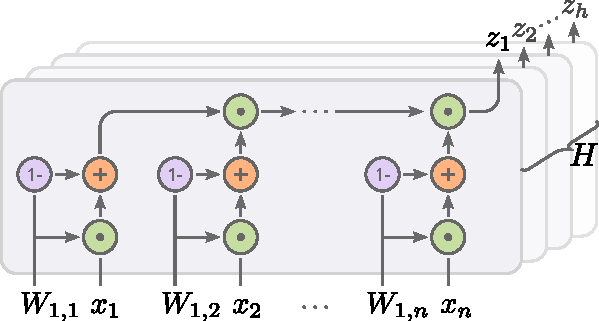
\includegraphics[scale=0.7]{graphics/nmu.pdf}
\caption{Visualization of NMU for a single output scalar $z_1$, this construction repeats for every element in the output vector $\mathbf{z}$.}
\end{figure}

\subsection{Learning a 10 parameter function}
Consider the static function $t = (x_1 + x_2) \cdot (x_1 + x_2 + x_3 + x_4)$ for $x \in \mathbb{R}^4$. To illustrate the ability of $\mathrm{NAC}_{\bullet}$, NALU, and our proposed NMU, we conduct 100 experiemnts for each model, where we attempt to fit this function. Table \ref{tab:very-simple-function-results} show that NMU has a higher success rate and converges faster.
%When inspecting the $6\%$ that did not converge, we found the issue to be underflow when $w = 0$ in the multiplication layer.
\begin{table}[!h]

\caption{\label{tab:very-simple-function-results}Shows the success-rate, at what global step the model converged at, and the sparsity error for all weight matrices, with 95\% confidence interval. Best result is highlighed.}
\centering
\begin{tabular}{crllll}
\toprule
\multicolumn{1}{c}{Op} & \multicolumn{1}{c}{Model} & \multicolumn{1}{c}{Success} & \multicolumn{2}{c}{Solved at} & \multicolumn{1}{c}{Sparsity error} \\
\cmidrule(l{3pt}r{3pt}){1-1} \cmidrule(l{3pt}r{3pt}){2-2} \cmidrule(l{3pt}r{3pt}){3-3} \cmidrule(l{3pt}r{3pt}){4-5} \cmidrule(l{3pt}r{3pt}){6-6}
 &  & Rate & Median & Mean & Mean\\
\midrule
 & $\mathrm{NAC}_{\bullet}$ & $13\% {~}^{+8\%}_{-5\%}$ & $5.5 \cdot 10^{4}$ & $5.9 \cdot 10^{4} {~}^{+7.8 \cdot 10^{3}}_{-6.6 \cdot 10^{3}}$ & $7.5 \cdot 10^{-6} {~}^{+2.0 \cdot 10^{-6}}_{-2.0 \cdot 10^{-6}}$\\

 & NALU & $26\% {~}^{+9\%}_{-8\%}$ & $7.0 \cdot 10^{4}$ & $7.8 \cdot 10^{4} {~}^{+6.2 \cdot 10^{3}}_{-8.6 \cdot 10^{3}}$ & $9.2 \cdot 10^{-6} {~}^{+1.7 \cdot 10^{-6}}_{-1.7 \cdot 10^{-6}}$\\

\multirow{-3}{*}{\centering\arraybackslash $\bm{\times}$} & NMU & $\mathbf{94\%} {~}^{+3\%}_{-6\%}$ & $\mathbf{1.4 \cdot 10^{4}}$ & $\mathbf{1.4 \cdot 10^{4}} {~}^{+2.2 \cdot 10^{2}}_{-2.1 \cdot 10^{2}}$ & $\mathbf{2.6 \cdot 10^{-8}} {~}^{+6.4 \cdot 10^{-9}}_{-6.4 \cdot 10^{-9}}$\\
\bottomrule
\end{tabular}
\end{table}


\section{Introducing differentiable binary arithmetic operations}
\label{sec:Nalu}
We define our problem as learning a set of static arithmetic operations between selected elements of a vector. E.g. for a vector $\mathbf{x}$ learn the function ${(x_5 + x_1) \cdot x_7}$. The approach taking in this paper, is to develop layers around specific operations, and then let each layer decide which inputs to include using backpropergation.

We develop these layers by analysing the theoretical issues in the Neural Arithmetic Logic Unit (NALU) by \citet{trask-nalu}.
s
\subsection{Introducing NALU}
The Neural Arithmetic Logic Unit (NALU) consists of two sub-units; the $\text{NAC}_{+}$ and $\text{NAC}_{\bullet}$. These exclusively represent either the $\{+, -\}$ or the $\{\times, \div \}$ operations. The NALU then assumes that either $\text{NAC}_{+}$ or $\text{NAC}_{\bullet}$ will be selected exclusively, using a sigmoid gating-mechanism.

The $\text{NAC}_{+}$ and $\text{NAC}_{\bullet}$ are defined accordingly,
\begin{align}
W_{h_\ell, h_{\ell-1}} &= \tanh(\hat{W}_{h_\ell, h_{\ell-1}}) \sigma(\hat{M}_{h_\ell, h_{\ell-1}}) \label{eq:weight}\\
\textrm{NAC}_+:\ z_{h_\ell} &= \sum_{h_{\ell-1}=1}^{H_{\ell-1}} W_{h_{\ell}, h_{\ell-1}} z_{h_{\ell-1}} \label{eq:naca}\\
\textrm{NAC}_\bullet:\ z_{h_\ell} &= \exp\left(\sum_{h_{\ell-1}=1}^{H_{\ell-1}} W_{h_{\ell}, h_{\ell-1}} \label{eq:nacm}\log(|z_{h_{\ell-1}}| + \epsilon) \right)
\end{align}
where $\hat{\mathbf{W}}, \hat{\mathbf{M}} \in \mathbb{R}^{H_{\ell} \times H_{\ell-1}}$ are weight matrices and $z_{h_{\ell-1}}$ is the input. The matrices are combined using a tanh-sigmoid transformation to bias the parameters towards a $\{-1,0,1\}$ solution. Having $\{-1,0,1\}$ allows $\text{NAC}_{+}$ to be perform exact $\{+, -\}$ operations between elements of a vector.
The $\text{NAC}_{\bullet}$ uses an exponential-log transformation to create the $\{\times, \div \}$ operations (within $\epsilon$ precision).

The NALU combines these units with a gating mechanism $\mathbf{z} = \mathbf{g} \odot \text{NAC}_{+} + (1 - \mathbf{g}) \odot \text{NAC}_{\bullet}$ given $\mathbf{g} = \sigma(\mathbf{G} \mathbf{x})$. Thus allowing NALU to decide between all of $\{+, -, \times, \div\}$ using backpropagation.

\subsection{Challenges of gating between \texorpdfstring{$\text{NAC}_{+}$}{NAC-add} and \texorpdfstring{$\text{NAC}_{\bullet}$}{NAC-mul}}
\label{sec:methods:gatting-issue}
The purpose of the gating-mechanism is to select either $\text{NAC}_{+}$ or $\text{NAC}_{\bullet}$ exclusively. This assumes that the correct sub-unit is selected in first try, since selecting the wrong sub-unit makes it impossible for the correct sub-unit to converge, as it is multiplied by zero.

This assumption is problematic as it rarely holds. The gating-mechanism will converge to select the $\text{NAC}_{+}$ unit, independently of the desired operation, as this unit is much easier to optimize and will thus be the best estimator early on. NALU works around this issue by sharing the weight matrix between $\text{NAC}_{+}$ and $\text{NAC}_{\bullet}$, such that even if $\text{NAC}_{+}$ is selected the weights can still, by pure chance, converge such that $\text{NAC}_{\bullet}$ is the best estimator.

To summarize, sharing the weight matrix allows, for a lucky seed, $\text{NAC}_{\bullet}$ to be selected. However, it also makes $\text{NAC}_{+}$ much harder to optimize when addition is the desired operation. We confirm this empirically in appendix \ref{sec:appendix:nalu-gate-experiment}, by comparing the NALU model with seperate and shared weights. Solving this problem is a research project on its own, we thus focus on improving the sub-units by assuming that the gating is known.

%To simplify the problem we have chosen to leave out the gating mechanism and focus on the sub-units, assuming "oracle gating". The gating mechanism of the NALU is difficult to converge, as shown in table \ref{tab:function-task-static-defaults}. This is likely due to the vastly different convergence properties. The independence in addition is a lot easier to learn than the heavily dependent multiplication operations, even for problems where addition is not the desired operation. Because addition converges faster, it becomes the best estimator early on and the gate will then choose addition. This causes the multiplication unit to be completely ignored, making it impossible for it to converge even if it is the desired operation.

\subsubsection{Weight matrix construction}\label{sssec:weight}

\citet{glorot-initialization} show that $E[z_{h_\ell}] = 0$ at initialization is a desired property, as it prevents explosion of both the output and the gradients. To satisfy this property with $W_{h_{\ell-1},h_\ell} = \tanh(\hat{W}_{h_{\ell-1},h_\ell}) \sigma(\hat{M}_{h_{\ell-1},h_\ell})$, an initialization must satisfy $E[\tanh(\hat{W}_{h_{\ell-1},h_\ell})] = 0$. In the context of NALU, this initialization is also unbiased as it samples evenly between $+$ and $-$, or $\times$ and $\div$. Unfortunately, this initialization also causes the expectation of the gradient to become zero, as show in \eqref{eq:nac-weight-gradient}.

\begin{equation}
E\left[\frac{\partial \mathcal{L}}{\partial \hat{M}_{h_{\ell-1},h_\ell}}\right] = E\left[\frac{\partial \mathcal{L}}{\partial W_{h_{\ell-1},h_\ell}}\right] E\left[\tanh(\hat{W}_{h_{\ell-1},h_\ell})\right] E\left[\sigma'(\hat{M}_{h_{\ell-1},h_\ell})\right] = 0
\label{eq:nac-weight-gradient}
\end{equation}

Besides the issue of initialization, our empirical analysis (table \ref{tab:function-task-static-defaults}) show that this weight construction \eqref{eq:weight} does not create the desired bias for $\{-1, 0, 1\}$ for the addition and subtraction problem.

To solve these issues, we add a sparsifying regularizer to the loss function ($\mathcal{L} = \hat{\mathcal{L}} + \lambda_{\mathrm{sparse}} \mathcal{R}_{\ell,\mathrm{sparse}}$) and use simple linear weight construction, where $W_{h_{\ell-1},h_\ell}$ is clamped to $[-1, 1]$ in each iteration.

\begin{align}
W_{h_{\ell-1},h_\ell} &= \min(\max(W_{h_{\ell-1},h_\ell}, -1), 1), \\
\mathcal{R}_{\ell,\mathrm{sparse}} &= \frac{1}{H_\ell \cdot H_{\ell-1}} \sum_{h_\ell=1}^{H_\ell} \sum_{h_{\ell-1}=1}^{H_{\ell-1}} \min\left(|W_{h_{\ell-1},h_\ell}|, 1 - \left|W_{h_{\ell-1},h_\ell}\right|\right) \\
\textrm{NAU}:\ z_{h_\ell} &= \sum_{h_{\ell-1}=1}^{H_{\ell-1}} W_{h_{\ell}, h_{\ell-1}} z_{h_{\ell-1}}
\end{align}

\subsubsection{Challenges of division} \label{sssec:nac-mul}

The $\text{NAC}_{\bullet}$, as formulated in equation \ref{eq:nacm}, has the ability to perform exact multiplication and division, or more precisely multiplication of the inverse of elements from a vector, when a weight in $W_{h_{\ell-1},h_\ell}$ is $-1$.

However, this flexibility creates critical optimization challenges. Expanding the exp-log-transformation, $\text{NAC}_{\bullet}$ can be express as
\begin{equation}
\textrm{NAC}_\bullet:\ z_{h_\ell} = \prod_{h_{\ell-1}=1}^{H_{\ell-1}} (|z_{h_{\ell-1}}| + \epsilon)^{W_{h_{\ell}, h_{\ell-1}}}\ .
\label{eq:division:nac-mul-rewrite}
\end{equation}

Equation \eqref{eq:division:nac-mul-rewrite} reveals that if $|z_{h_{\ell-1}}|$ is near zero (which is likely since $E[z_{h_{\ell-1}}] = 0$ is a desired property when initializing \cite{glorot-initialization}), $W_{h_{\ell-1},h_\ell}$ is negative, and $\epsilon$ is small, then the output will explode. This issue is present even for a reasonably large $\epsilon$ value (such as $\epsilon = 0.1$), and just a slightly negative $W_{h_{\ell-1},h_\ell}$, as visualized in figure \ref{fig:nac-mul-eps-issue}. Also note that the curvature can cause convergence to an unstable area.

This singularity issue, is present even when multiplication is the desired operation. Since a multiplication unit should not explode for $z_{h_{\ell-1}}$ near zero, it is likely that  supporting division is infeasible. The NALU paper shows the same difficulty, as they are unable to learn division on the interpolation range. Their results on the extrapolation range is an artifact of their evaluation method.

%However, backpropagation through the $\text{NAC}_{\bullet}$ unit (equation \ref{eq:dz}, derivation in Appendix \ref{sec:appendix:gradient-derivatives:gradient-nac-mul}) reveals that if $|z_{h_{\ell-1}}|$ is near zero, $W_{h_{\ell-1},h_\ell}$ is negative and $\epsilon$ is small, the gradient term will explode and oscillate between large positive and large negative values, which can be problematic in optimization \cite{adam-optimization}, as visualized in figure \ref{fig:nac-mul-eps-issue}.
%\begin{align}
%\frac{\partial \mathcal{L}}{\partial W_{h_{\ell}, h_{\ell - 1}}} &= \frac{\partial \mathcal{L}}{\partial z_{h_\ell}} \frac{\partial z_{h_\ell}}{\partial W_{h_{\ell}, h_{\ell - 1}}} = \frac{\partial \mathcal{L}}{\partial z_{h_\ell}} z_{h_\ell} \log(|z_{h_{\ell-1}}| + \epsilon) \label{eq:dw}\\
%\frac{\partial \mathcal{L}}{\partial z_{h_{\ell-1}}} &= \sum_{h_\ell = 1}^{H_\ell} \frac{\partial \mathcal{L}}{\partial z_{h_\ell}} \frac{\partial z_{h_\ell}}{\partial z_{h_{\ell-1}}} = \sum_{h_\ell = 1}^{H_\ell} \frac{\partial \mathcal{L}}{\partial z_{h_\ell}} z_{h_\ell} W_{h_\ell, h_{\ell-1}} \frac{\mathrm{sign}(z_{h_{\ell-1}})}{|z_{h_{\ell-1}}| + \epsilon}\label{eq:dz}
%\end{align}

%This is not an issue for positive values of $W_{h_{\ell-1},h_\ell}$ (multiplication), as $z_{h_{\ell}}$ and $z_{h_{\ell-1}}$ will be correlated causing the terms $z_{h_\ell}$ and $\frac{\mathrm{sign}(z_{h_{\ell-1}})}{|z_{h_{\ell-1}}| + \epsilon}$ to partially cancel out.

% This gradient can be particular problematic when considering that $E[z_{h_{\ell-1}}] = 0$ is a desired property when initializing \cite{glorot-initialization}.
% A desired multiplication unit should not explode for $z_{h_{\ell-1}}$ near zero, which is why supporting division is likely infeasible.

\begin{figure}[h]
\centering
\begin{subfigure}{.33\textwidth}
  \centering
  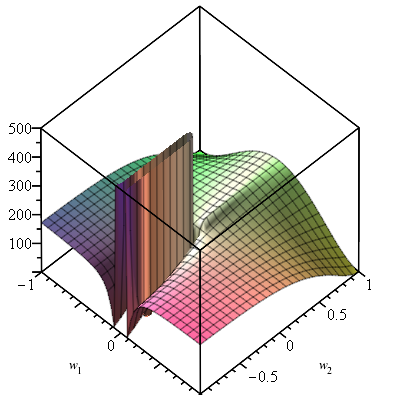
\includegraphics[width=\linewidth,trim={0 0 0 4.35cm},clip]{graphics/nac-mul-eps-1em7.png}
  \caption{$\mathrm{NAC}_{\bullet}$ with $\epsilon = 10^{-7}$}
\end{subfigure}%
\begin{subfigure}{.33\textwidth}
  \centering
  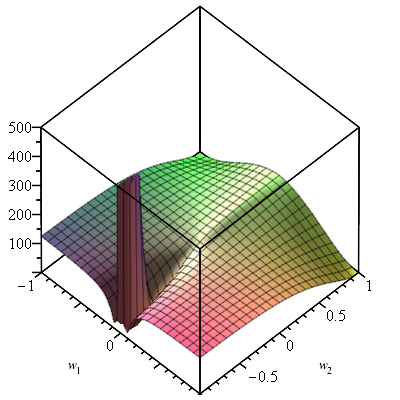
\includegraphics[width=\linewidth,trim={0 0 0 4.35cm},clip]{graphics/nac-mul-eps-1em1.png}
  \caption{$\mathrm{NAC}_{\bullet}$ with $\epsilon = 0.1$}
\end{subfigure}
\begin{subfigure}{.33\textwidth}
  \centering
  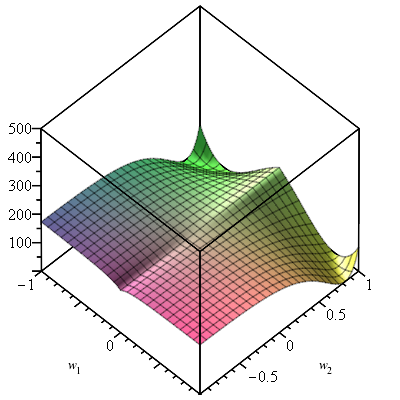
\includegraphics[width=\linewidth,trim={0 0 0 4.35cm},clip]{graphics/nac-mul-eps-1.png}
  \caption{$\epsilon = 1$}
\end{subfigure}
%\begin{subfigure}{.33\textwidth}
%  \centering
%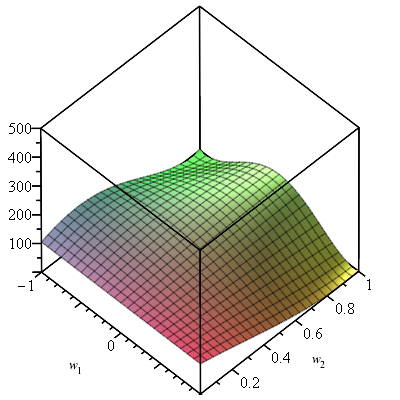
\includegraphics[width=\linewidth]{graphics/nac-mul-nmu.png}
%  \caption{Our NMU solution}
%\end{subfigure}

\caption{RMS loss curvature for a $\mathrm{NAC}_{+}$ layer followed by either a $\mathrm{NAC}_{\bullet}$. The weight matrices constrained are to $\mathbf{W}_1 = \left[\protect\begin{smallmatrix}
w_1 & w_1 & 0 & 0 \\
w_1 & w_1 & w_1 & w_1
\protect\end{smallmatrix}\right]$, $\mathbf{W}_2 = \left[\protect\begin{smallmatrix}
w_2 & w_2
\protect\end{smallmatrix}\right]$. The problem is $(x_1 + x_2) \cdot (x_1 + x_2 + x_3 + x_4)$ for $x = \left(1, 1.2, 1.8, 2\right)$. The desired solution is $w_1 = w_2 = 1$, although this problem have additional undesired unstable solutions.}
\label{fig:nac-mul-eps-issue}
\end{figure}

\subsubsection{Initialization of \texorpdfstring{$\mathrm{NAC}_{\bullet}$}{NAC-mul}}
Initialization is important to consider for fast and consistent convergence, one desired property is that weights can be initialized such that $E[z_{h_\ell}] = 0$ \cite{glorot-initialization}. Using second order Taylor approximation and assuming all $z_{h_{\ell-1}}$ are uncorrelated, the expectation of $\mathrm{NAC}_{\bullet}$ can be estimated as
\begin{equation}
E[z_{h_\ell}] \approx \left(1 + \frac{1}{2} Var[W_{h_\ell, h_{\ell-1}}] \log(|E[z_{h_{\ell-1}}]| + \epsilon)^2\right)^{H_{\ell-1}} \Rightarrow E[z_{h_\ell}] > 1.
\label{eq:nac-mul:expectation}
\end{equation}
As shown in equation \ref{eq:nac-mul:expectation}, satisfying $E[z_{h_\ell}] = 0$ for $\mathrm{NAC}_{\bullet}$ is likely impossible. The variance can also not be input-independent initialized and is expected to explode (proofs in Appendix \ref{sec:appendix:moments:nac-mul}).

\subsubsection{Neural multiplication unit}
To solve the the gradient and initialization challenges for $\mathrm{NAC}_{\bullet}$ we propose a new neural multiplication unit (NMU):

\begin{align}
W_{h_{\ell-1},h_\ell} &= \min(\max(W_{h_{\ell-1},h_\ell}, 0), 1), \\
\mathcal{R}_{\ell,\mathrm{sparse}} &= \frac{1}{H_\ell \cdot H_{\ell-1}} \sum_{h_\ell=1}^{H_\ell} \sum_{h_{\ell-1}=1}^{H_{\ell-1}} \min\left(W_{h_{\ell-1},h_\ell}, 1 - W_{h_{\ell-1},h_\ell}\right) \\
\textrm{NMU}:\ z_{h_\ell} &= \prod_{h_{\ell-1}=1}^{H_{\ell-1}} \left(W_{h_{\ell-1},h_\ell} z_{h_{\ell-1}} + 1 - W_{h_{\ell-1},h_\ell} \right) \label{eq:nmu-defintion}
\end{align}
The NMU is regularized similar to the NAU and has a multiplicative identity when $W_{h_{\ell-1},h_\ell}=0$.
The NMU unit does not support division by design.
%Previous experiments using the NALU for division does not work well on division hence very little is lost with this modification \cite{trask-nalu}.
As opposed to the $\mathrm{NAC}_{\bullet}$, the NMU can represent input of both negative and positive values and is not $\epsilon$ bounded, which allows the NMU to extrapolate to $z_{h_{\ell-1}}$ that are negative or smaller than $\epsilon$. Its gradients are derived in Appendix \ref{sec:appendix:gradient-derivatives:gradient-nmu}.

\subsubsection{Moments and initialization}
Our proposed NAU can be initialized using Glorot initialization as it is a linear layer. The $\mathrm{NAC}_{+}$ unit can also achieve an ideal initialization, although it is less trivial (details in Appendix \ref{sec:appendix:moments:weight-matrix-construction}).

Our proposed NMU is initialized with $E[W_{h_{\ell}, h_{\ell - 1}}] = \nicefrac{1}{2}$. Assuming all $z_{h_{\ell-1}}$ are uncorrelated, and $E[z_{h_{\ell-1}}] = 0$, which is the case for most units, the expectation can be approximated to
\begin{equation}
E[z_{h_\ell}] \approx \left(\frac{1}{2}\right)^{H_{\ell-1}},
\end{equation}
which approaches zero for $H_{\ell-1} \rightarrow \infty$ (see Appendix \ref{sec:appendix:moments:nmu}). The NMU can, assuming $Var[z_{h_{\ell-1}}] = 1$ and $H_{\ell-1}$ is large, be initialized optimally with $Var[W_{h_{\ell-1},h_\ell}] = \frac{1}{4}$ (proof in Appendix \ref{sec:appendix:moments:nmu:initialization}).

\subsubsection{Regularizer scaling}
We use the regularizer scaling as defined in \eqref{eq:regualizer-scaling}. The motivation here, is that the optimization consists of two parts. A warmup period, where $W_{h_{\ell-1},h_\ell}$ should get close to the solution, unhindered by the sparsity regularizer, and then a period where the solution is made sparse.
\begin{equation}
\lambda_{\mathrm{sparse}} = \hat{\lambda}_{\mathrm{sparse}} \max\left(\min\left(\frac{t - \lambda_{\mathrm{start}}}{\lambda_{\mathrm{end}} - \lambda_{\mathrm{start}}}, 1\right), 0\right)
\label{eq:regualizer-scaling}
\end{equation}

\section{Related work}
Pure neural models that learns arithmetic tasks through backpropagation have previously been attempted.
They either utilize convolutions, gating, differentiable memory, and/or attention architectures \cite{NeuralGPU,GridLSTM,NTM}.
Some of the results have close to perfect extrapolation. However, the models are constrained to work only on whole numbers and requires well defined arithmetic setups such as binary representations of numbers for input and output.
We do not test the expressiveness of current approximate approaches, but instead develop a fundamental new unit of computation with weight constraints to learn exact arithmetic operations that works on real numbers, without any assumptions of binary representations.

To handle operations on real numbers, the Neural Arithmetic Expression Calculator \cite{NAEC} propose learning the individual components needed.
They repeatedly combine program induction with a memory-encoder-decoder architecture trained with reinforcement learning.
While this model has the ability to dynamically handle a larger variety of expressions compared to our solution, they do not generalize much beyond interpolation length.

We use the NAU to do a subset-selection, which is then followed by either a summation or multiplication, in order to combine information from the input vector.
An alternative, fully differentiable version, is to use a gumbel-softmax to perform exact subset-selection \cite{DSS}.
This, however, has the restriction of having to use a predefined size of the subset, which is a strong assumption that our units are not limited by.

\section{Experimental results}
\label{sec:experiments}

\subsection{Arithmetic datasets}
\label{sec:arithmetic-dataset}

The arithmetic dataset is a replica of the "simple function task" as shown in \cite{trask-nalu}.
The goal is to sum two random subsets of a vector and perform a arithmetic operation as defined below
\begin{equation}
t = \sum_{i = s_{1,\mathrm{start}}}^{s_{1,\mathrm{end}}} x_i \circ \sum_{i = s_{2,\mathrm{start}}}^{s_{2,\mathrm{end}}} x_i \quad \text{where } \mathbf{x} \in \mathbb{R}^n, x_i \sim \mathrm{Uniform}[r_{\mathrm{lower}}, r_{\mathrm{upper}}], \circ \in \{+, -, \times\}
\label{eq:arithmetic-problem}
\end{equation}
where $n$ (default $100$), $U[r_{\mathrm{lower}}, r_{\mathrm{upper}}]$ (interpolation default is $U[1,2]$ and extrapolation default is $U[2,6]$), the subset size (default 25\%), and subset overlap (default 50\%) are parameters that we use to assess learning capability (see details in appendix \ref{sec:appendix:simple-function-task:data-generation} and the effect of varying the parameters in appendix \ref{sec:appendix-simple-function-task:dataset-parameter-effect}).

\subsubsection{Model evaluation}
The goal is to achieve a solution that is acceptably close to a perfect solution. To evaluate if a model instance solves the task consistently we compare the MSE to a nearly-perfect solution on the extrapolation range over multiple seeds. If $\mathbf{W}_1, \mathbf{W}_2$ defines the weights of the fitted model, and $\mathbf{W}_1^\epsilon$ is nearly-perfect and $\mathbf{W}_2^*$ is perfect (example in equation \ref{eq:nearly-perfect-solution-example}), the success criteria is $\mathcal{L}_{\mathbf{W}_1, \mathbf{W}_2} < \mathcal{L}_{\mathbf{W}_1^\epsilon, \mathbf{W}_2^*}$, measured on the extrapolation error, for $\epsilon = 10^{-5}$.
\begin{equation}
    \mathbf{W}_1^\epsilon = \begin{bmatrix}
    1 - \epsilon & 1 - \epsilon & 0 + \epsilon & 0 + \epsilon \\
    1 - \epsilon & 1 - \epsilon & 1 - \epsilon & 1 - \epsilon
    \end{bmatrix}, \mathbf{W}_2^* = \begin{bmatrix}
    1 & 1
    \end{bmatrix}
    \label{eq:nearly-perfect-solution-example}
\end{equation}
To measure speed of convergence the first iteration for which $\mathcal{L}_{\mathbf{W}_1, \mathbf{W}_2} < \mathcal{L}_{\mathbf{W}_1^\epsilon, \mathbf{W}_2^*}$ is reported with a 95\% confidence interval. Only models that managed to solve the task are included.

We assume an approximate discrete solution with parameters close to $\{-1, 0, 1\}$ is important for inferring exact arithmetic operations.
To measure the sparsity we introduce a sparsity error (defined in equation \ref{eq:sparsity-error}).
Similar to the convergence metric we only considered model instances that did solve the task and report the 95\% confidence interval.
\begin{equation}
E_\mathrm{sparsity} = \max_{h_{\ell-1}, h_{\ell}} \min(|W_{h_{\ell-1},h_\ell}|, |1 - |W_{h_{\ell-1},h_\ell}||)
\label{eq:sparsity-error}
\end{equation}

We evaluate each metric every $1000$ iterations on the test set that uses the extrapolation range, and choose the best iteration based on the validation dataset that uses the interpolation range.

\subsubsection{Arithmetic operation comparison}
We compare models on different arithmetic operation $\circ \in \{+, -, \times\}$. The multiplication models, NMU and $\mathrm{NAC}_{\bullet}$, have an addition layer first, either NAU or $\mathrm{NAC}_{+}$, followed by a multiplication layer. The addition models are just two layers of the same unit. Finally, the NALU model consists of two NALU layers. See explicit definitions in appendix \ref{sec:appendix:comparison-all-models}.

Each experiment is trained for $5 \cdot 10^6$ iterations (details in appendix \ref{sec:appendix:comparison-all-models}). Results are presented in table \ref{tab:function-task-static-defaults}. For multiplication, the NMU succeeds more often and converges faster. For addition and subtraction, the NAU model converges faster, given the median, and has a sparser solution. A larger comparison is in appendix \ref{sec:appendix:comparison-all-models} and an ablation study is in appendix \ref{sec:appendix:ablation-study}.

\begin{table}[!h]

\caption{\label{tab:function-task-static-defaults}Shows the success-rate for $\mathcal{L}_{\mathbf{W}_1, \mathbf{W}_2} < \mathcal{L}_{\mathbf{W}_1^\epsilon, \mathbf{W}_2^*}$, at what global step the model converged at, and the sparsity error for all weight matrices.}
\centering
\begin{tabular}{crllll}
\toprule
\multicolumn{1}{c}{Op} & \multicolumn{1}{c}{Model} & \multicolumn{1}{c}{Success} & \multicolumn{2}{c}{Solved at} & \multicolumn{1}{c}{Sparsity error} \\
\cmidrule(l{3pt}r{3pt}){1-1} \cmidrule(l{3pt}r{3pt}){2-2} \cmidrule(l{3pt}r{3pt}){3-3} \cmidrule(l{3pt}r{3pt}){4-5} \cmidrule(l{3pt}r{3pt}){6-6}
 &  & Rate & Median & Mean & Mean\\
\midrule
 & $\mathrm{NAC}_{\bullet}$ & $30\%$ & $2.5 \cdot 10^{6}$ & $2.5 \cdot 10^{6} \pm 1.5 \cdot 10^{6}$ & $\mathbf{3.9 \cdot 10^{-4} \pm 9.4 \cdot 10^{-4}}$\\

 & Linear & $0\%$ & --- & --- & ---\\

 & NALU & $0\%$ & --- & --- & ---\\

\multirow{-4}{*}{\centering\arraybackslash $\bm{\times}$} & NMU & $\mathbf{90\%}$ & $\mathbf{1.4 \cdot 10^{6}}$ & $\mathbf{1.6 \cdot 10^{6} \pm 5.6 \cdot 10^{5}}$ & $1.8 \cdot 10^{-3} \pm 1.1 \cdot 10^{-3}$\\
\cmidrule{1-6}
 & $\mathrm{NAC}_{+}$ & $\mathbf{100\%}$ & $6.0 \cdot 10^{4}$ & $7.1 \cdot 10^{4} \pm 2.4 \cdot 10^{4}$ & $4.8 \cdot 10^{-1} \pm 2.0 \cdot 10^{-2}$\\

 & Linear & $\mathbf{100\%}$ & $4.2 \cdot 10^{4}$ & $\mathbf{4.2 \cdot 10^{4} \pm 1.9 \cdot 10^{3}}$ & $6.1 \cdot 10^{-1} \pm 1.2 \cdot 10^{-1}$\\

 & NALU & $0\%$ & --- & --- & ---\\

\multirow{-4}{*}{\centering\arraybackslash $\bm{+}$} & NAU & $\mathbf{100\%}$ & $\mathbf{1.8 \cdot 10^{4}}$ & $7.0 \cdot 10^{5} \pm 9.2 \cdot 10^{5}$ & $\mathbf{1.7 \cdot 10^{-3} \pm 8.0 \cdot 10^{-4}}$\\
\cmidrule{1-6}
 & $\mathrm{NAC}_{+}$ & $\mathbf{100\%}$ & $8.0 \cdot 10^{3}$ & $1.5 \cdot 10^{6} \pm 1.5 \cdot 10^{6}$ & $4.6 \cdot 10^{-1} \pm 2.9 \cdot 10^{-2}$\\

 & Linear & $\mathbf{100\%}$ & $1.1 \cdot 10^{6}$ & $1.9 \cdot 10^{6} \pm 1.3 \cdot 10^{6}$ & $3.7 \cdot 10^{-1} \pm 1.1 \cdot 10^{-1}$\\

 & NALU & $20\%$ & $3.6 \cdot 10^{6}$ & $3.6 \cdot 10^{6} \pm 1.3 \cdot 10^{7}$ & $4.7 \cdot 10^{-1} \pm 3.3 \cdot 10^{-1}$\\

\multirow{-4}{*}{\centering\arraybackslash $\bm{-}$} & NAU & $\mathbf{100\%}$ & $\mathbf{4.0 \cdot 10^{3}}$ & $\mathbf{4.2 \cdot 10^{3} \pm 3.0 \cdot 10^{2}}$ & $\mathbf{1.9 \cdot 10^{-3} \pm 4.2 \cdot 10^{-4}}$\\
\bottomrule
\end{tabular}
\end{table}


\subsubsection{Evaluating theoretical claims}

To validate our theoretical claim, that the NMU models works better than $NAC_{\bullet}$ for larger $H_{\ell-1}$, we increase the hidden size of the network, thereby adding redundant units. Redundant units are very common neural networks, where the purpose is to fit an unknown function.

Additionally, the NMU model is unlike the $NAC_{\bullet}$ model also capable of understanding inputs that are both negative and positive. To validate this empirically, the training and validation datasets are sampled for $\mathrm{U}[-2,2]$, and then tested on $\mathrm{U}[-6,-2] \cup \mathrm{U}[2,6]$.

Finally, to validate that division and the lack of bias in $NAC_{\bullet}$ are critical issues but that solving these alone are not enough, two additional models compared with. A variant of $\mathrm{NAC}_{\bullet}$ called $\mathrm{NAC}_{\bullet, \sigma}$, that only supports multiplication, by constraining the weights with $W = \sigma(\hat{W})$. And a variant, called $\mathrm{NAC}_{\bullet, \mathrm{NMU}}$, that uses linear weights and bias regularization, identically to that in NMU model.

Figure \ref{fig:simple-function-static-theoreical-claims-experiment} shows that the NMU can both handle a much larger hidden-size, as well as negative inputs, and that solving the division and bias issues alone improves the success rate, but are no enough when the hidden-size is large, as there is no ideal initialization.

\begin{figure}[h]
\centering
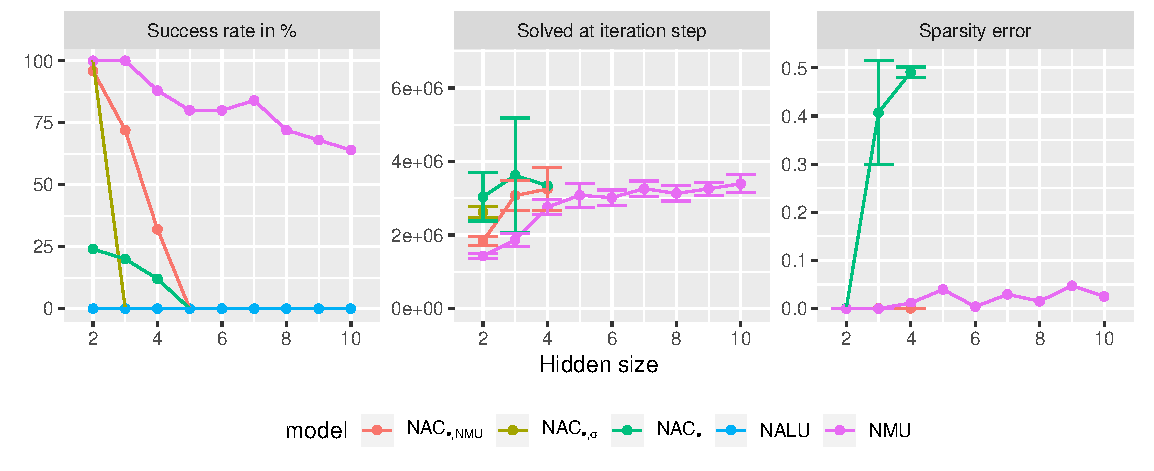
\includegraphics[width=\linewidth,trim={0 1.3cm 0 0},clip]{results/simple_function_static_mul_hidden_size.pdf}
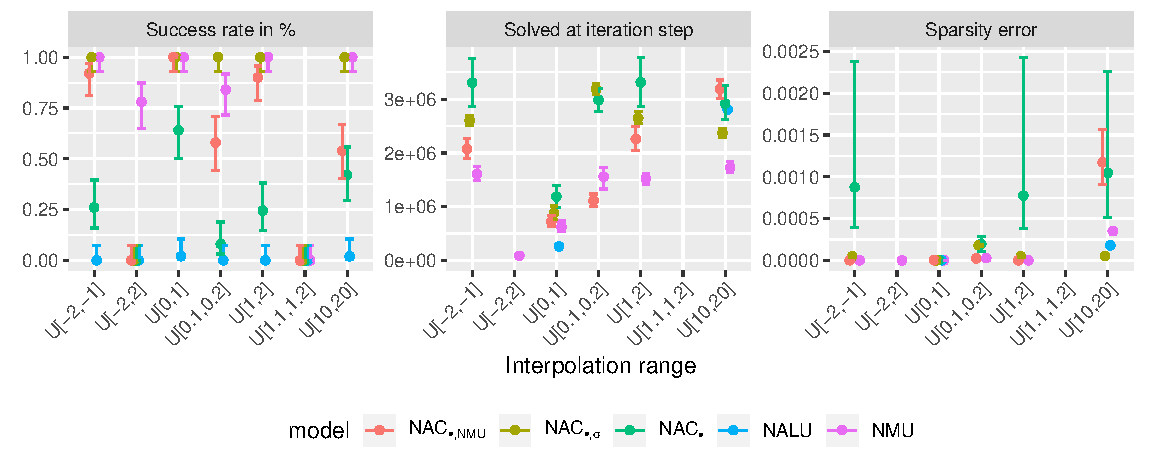
\includegraphics[width=\linewidth,trim={0 0 0 0.809cm},clip]{results/simple_function_static_mul_range.pdf}
\caption{Shows that the NMU can handle a large hidden size, and works when the input contains both positive and negative numbers ($U[-2,-2]$).} 
%\caption{Shows the effect of the dataset parameters. For each interpolation range, the following extrapolation ranges are used: ${\mathrm{U}[-2,2] \rightarrow \mathrm{U}[-6,-2] \cup \mathrm{U}[2,6]}$, ${\mathrm{U}[0,1] \rightarrow \mathrm{U}[1,5]}$, ${\mathrm{U}[0.1,0.2] \rightarrow \mathrm{U}[0.2,2]}$, ${\mathrm{U}[1,2] \rightarrow \mathrm{U}[2,6]}$, ${\mathrm{U}[10, 20] \rightarrow \mathrm{U}[20, 40]}$. The uniform sampling ranges are chosen to test the effect of mean, variance, and sign for optimizing.}
\label{fig:simple-function-static-theoreical-claims-experiment}
\end{figure}

\subsection{Product of sequential MNIST}

To compare how easy it is to backpropergation though the arithmetic layers, the arithmetic layers are applied as a recurrent-unit to a sequence of MNIST digits, where the target is to fit the cumulative product. This task is similar to ``MNIST Counting and Arithmetic Tasks'' in \cite{trask-nalu}\footnote{Also uses the same CNN, \url{https://github.com/pytorch/
examples/tree/master/mnist}.}, but use multiplication rather than addition.. Each model is trained on sequences of length 2, and then tested on sequences of length 20 MNIST digits.

Success of convergence is determined by comparing the MSE of each model, with a baseline model that directly computes the sequential product. If the MSE of each model, is less than the upper 1\% MSE-confidence-interval of the baseline model, then the model is considered successfully converged.

Sparsity and ``solved at iteration step'' is determined as described in experiment \ref{sec:arithmetic-dataset}. The validation set is the last 5000 MNIST digits from the training set, which is used to select the best epoch.

In this experiment we discovered that having an unconstrained ``input-network'' causes the multiplication-units to learn an undesired solution, such as $(0.1 \cdot 81 + 1 - 0.1) = 9$. This solves the problem with a similar success-rate, but not in the intended way. To prevent such solution, we regularize the CNN output with $\mathcal{R}_{\mathrm{z}} = \frac{1}{H_{\ell-1} H_\ell} \sum_{h_\ell}^{H_\ell} \sum_{h_{\ell-1}}^{H_{\ell-1}} (1 - W_{h_{\ell-1},h_\ell}) \cdot (1 - \bar{z}_{h_{\ell-1}})^2$. This regularizer is applied to the NMU and $\mathrm{NAC}_{\bullet,\mathrm{NMU}}$ models. See appendix \ref{sec:appendix:sequential-mnist:ablation} for the results, when this regularizer is not used.

Figure \ref{fig:sequential-mnist-prod-results} shows that the NMU does not hindre learning a more complex neural network. And that it can extrapolate to much longer sequences than what is is trained on.

\begin{figure}[h]
\centering
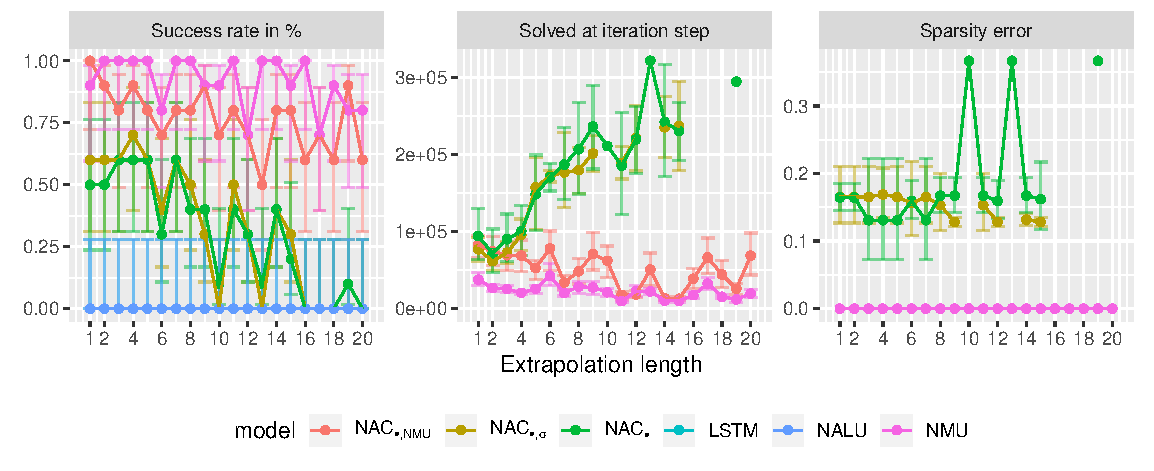
\includegraphics[width=\linewidth,trim={0 0.5cm 0 0},clip]{results/sequential_mnist_prod_long.pdf}
\caption{Shows the ability of each model to backpropergation and extrapolate to larger sequence lengths.} 
\label{fig:sequential-mnist-prod-results}
\end{figure}

\section{Conclusion}
By including theoretical considerations, such as initialization, gradients, and sparsity, we have developed a new multiplication unit that outperforms the state-of-the-art models on established extrapolation and sequential tasks. Our model converges more consistently, faster, and to more sparse solutions, than previously proposed models. 

We find that performing division and multiplication concurrently is a hard problem because of division by zero that currently can not be solved. However, when it comes to multiplication, our model is capable of extrapolating in both the negative range and to very small numbers.
%A theoretical disadvantage of our multiplication unit is that it is incapable of division. However, previous publications concur that this is a problematic and generally unsolved area, due to the singularity in division. Thus our proposed model is empirically identical when it comes to division. On the other hand, when it comes to multiplication, our model is capable of extrapolating in both the negative range and to very small numbers.

Finally, when it comes to considering more than just two inputs to the multiplication layer, our model clearly outperforms all previously proposed models as well as variations of previous models that borrow from our model. The ability for a neural layer to consider more than just two inputs, is critical in neural networks where the desired function is unknown.

\clearpage
\ifdefined\nonanonymous
\subsubsection*{Acknowledgments}
We would like to thank Andrew Trask and the other authors of the NALU paper, for highlighting the importance and challenges of extrapolation in Neural Networks. We would also like to thank the students Raja Shan Zaker Kreen and William Frisch Møller from The Technical University of Denmark, who initially showed us that the NALU do not converge consistently. 

This research is funded by the Innovation Foundation Denmark through the DABAI project.
\fi

\bibliographystyle{iclr2020_conference}
\bibliography{bibliography}

\newpage
\appendix
\section{Gradient derivatives}
\label{sec:appendix:gradient-derivatives}

\subsection{Weight matrix construction}
\label{sec:appendix:gradient-derivatives:weight-matrix-construction}
For clarity the weight matrix construction is defined using scalar notation
\begin{equation}
W_{h_\ell, h_{\ell-1}} = \tanh(\hat{W}_{h_\ell, h_{\ell-1}}) \sigma(\hat{M}_{h_\ell, h_{\ell-1}})
\end{equation}

The of the loss with respect to $\hat{W}_{h_\ell, h_{\ell-1}}$ and $\hat{M}_{h_\ell, h_{\ell-1}}$ is then straight forward to derive.
\begin{equation}
\begin{aligned}
\frac{\partial\mathcal{L}}{\partial \hat{W}_{h_\ell, h_{\ell-1}}} &= \frac{\partial\mathcal{L}}{\partial W_{h_\ell, h_{\ell-1}}} \frac{\partial W_{h_\ell, h_{\ell-1}}}{\partial \hat{W}_{h_\ell, h_{\ell-1}}} \\
&= \frac{\partial\mathcal{L}}{\partial W_{h_\ell, h_{\ell-1}}} (1 - \tanh^2(\hat{W}_{h_\ell, h_{\ell-1}})) \sigma(\hat{M}_{h_\ell, h_{\ell-1}}) \\
\frac{\partial\mathcal{L}}{\partial \hat{M}_{h_\ell, h_{\ell-1}}} &= \frac{\partial\mathcal{L}}{\partial W_{h_\ell, h_{\ell-1}}} \frac{\partial W_{h_\ell, h_{\ell-1}}}{\partial \hat{M}_{h_\ell, h_{\ell-1}}} \\
&= \frac{\partial\mathcal{L}}{\partial W_{h_\ell, h_{\ell-1}}} \tanh(\hat{W}_{h_\ell, h_{\ell-1}}) \sigma(\hat{M}_{h_\ell, h_{\ell-1}}) (1 - \sigma(\hat{M}_{h_\ell, h_{\ell-1}}))
\end{aligned}
\end{equation}

As seen from this result, one only needs to consider $\frac{\partial\mathcal{L}}{\partial W_{h_\ell, h_{\ell-1}}}$ for $\mathrm{NAC}_{+}$ and $\mathrm{NAC}_{\bullet}$, as the gradient with respect to $\hat{W}_{h_\ell, h_{\ell-1}}$ and $\hat{M}_{h_\ell, h_{\ell-1}}$ is just a multiplication on $\frac{\partial\mathcal{L}}{\partial W_{h_\ell, h_{\ell-1}}}$.

\subsection{Gradient of $\mathrm{NAC}_{\bullet}$}
\label{sec:appendix:gradient-derivatives:gradient-nac-mul}

First the $\textrm{NAC}_\bullet$ is defined using scalar notation.
\begin{equation}
z_{h_\ell} = \exp\left(\sum_{h_{\ell-1}=1}^{H_{\ell-1}} W_{h_{\ell}, h_{\ell-1}} \log(|z_{h_{\ell-1}}| + \epsilon) \right)
\end{equation}

The gradient of the loss with respect to $W_{h_\ell, h_{\ell-1}}$ is straight forward to derive.
\begin{equation}
\begin{aligned}
\frac{\partial z_{h_\ell}}{\partial W_{h_\ell, h_{\ell-1}}} &= \exp\left(\sum_{h'_{\ell-1}=1}^{H_{\ell-1}} W_{h_{\ell}, h'_{\ell-1}} \log(|z_{h'_{\ell-1}}| + \epsilon) \right) \log(|z_{h_{\ell-1}}| + \epsilon) \\
&= z_{h_\ell} \log(|z_{h_{\ell-1}}| + \epsilon)
\end{aligned}
\end{equation}

We now wish to derive the backpropagation term $\delta_{h_\ell} = \frac{\partial \mathcal{L}}{\partial z_{h_\ell}}$, because $z_{h_\ell}$ affects $\{z_{h_{\ell+1}}\}_{h_{\ell+1}=1}^{H_{\ell+1}}$ this becomes:
\begin{equation}
\delta_{h_\ell} = \frac{\partial \mathcal{L}}{\partial z_{h_\ell}} = \sum_{h_{\ell+1}=1}^{H_{\ell+1}} \frac{\partial \mathcal{L}}{\partial z_{h_{\ell+1}}} \frac{\partial z_{h_{\ell+1}}}{\partial z_{h_\ell}} = \sum_{h_{\ell+1}=1}^{H_{\ell+1}} \delta_{h_{\ell+1}} \frac{\partial z_{h_{\ell+1}}}{\partial z_{h_\ell}}
\end{equation}

To make it easier to derive $\frac{\partial z_{h_{\ell+1}}}{\partial z_{h_\ell}}$ we re-express the $z_{h_\ell}$ as $z_{h_{\ell+1}}$.
\begin{equation}
z_{h_{\ell+1}} = \exp\left(\sum_{h_{\ell}=1}^{H_{\ell}} W_{h_{\ell+1}, h_{\ell}} \log(|z_{h_{\ell}}| + \epsilon) \right)
\end{equation}

The gradient of $\frac{\partial z_{h_{\ell+1}}}{\partial z_{h_\ell}}$ is then:
\begin{equation}
\begin{aligned}
\frac{\partial z_{h_{\ell+1}}}{\partial z_{h_\ell}} &= \exp\left(\sum_{h_{\ell}=1}^{H_{\ell}} W_{h_{\ell+1}, h_{\ell}} \log(|z_{h_{\ell}}| + \epsilon) \right) W_{h_{\ell+1}, h_{\ell}} \frac{\partial \log(|z_{h_{\ell}}| + \epsilon)}{\partial z_{h_\ell}} \\
&= \exp\left(\sum_{h_{\ell}=1}^{H_{\ell}} W_{h_{\ell+1}, h_{\ell}} \log(|z_{h_{\ell}}| + \epsilon) \right) W_{h_{\ell+1}, h_{\ell}} \frac{\mathrm{abs}'(z_{h_{\ell}})}{|z_{h_{\ell}}| + \epsilon} \\
&= z_{h_{\ell+1}} W_{h_{\ell+1}, h_{\ell}} \frac{\mathrm{abs}'(z_{h_{\ell}})}{|z_{h_{\ell}}| + \epsilon} 
\end{aligned}
\end{equation}

$\mathrm{abs}'(z_{h_{\ell}})$ is the gradient of the absolute function. In the paper we denote this as $\mathrm{sign}(z_{h_{\ell}})$ for brevity. However, depending on the exact definition used there may be a difference for $z_{h_{\ell}} = 0$, as $\mathrm{abs}'(0)$ is undefined. In practicality this doesn't matter much though, although theoretically it does mean that the expectation of this is theoretically undefined when $E[z_{h_{\ell}}] = 0$.

\subsection{Gradient of NMU}
\label{sec:appendix:gradient-derivatives:gradient-nmu}

In scalar notation the NMU is defined as:
\begin{equation}
z_{h_\ell} = \prod_{h_{\ell-1}=1}^{H_{\ell-1}} \left(W_{h_{\ell-1},h_\ell} z_{h_{\ell-1}} + 1 - W_{h_{\ell-1},h_\ell} \right)
\end{equation}

The gradient of the loss with respect to $W_{h_{\ell-1},h_\ell}$ is fairly trivial. Note that every term but the one for $h_{\ell-1}$, is just a constant with respect to $W_{h_{\ell-1},h_\ell}$. The product, expect the term for $h_{\ell-1}$ can be expressed as $\frac{z_{h_\ell}}{W_{h_{\ell-1},h_\ell} z_{h_{\ell-1}} + 1 - W_{h_{\ell-1},h_\ell}}$. Using this fact, it becomes trivial to derive the gradient as:

\begin{equation}
\frac{\partial \mathcal{L}}{\partial w_{h_{\ell}, h_{\ell - 1}}} = \frac{\partial \mathcal{L}}{\partial z_{h_\ell}} \frac{\partial z_{h_\ell}}{\partial w_{h_{\ell}, h_{\ell - 1}}} = \frac{\partial \mathcal{L}}{\partial z_{h_\ell}} \frac{z_{h_\ell}}{W_{h_{\ell-1},h_\ell} z_{h_{\ell-1}} + 1 - W_{h_{\ell-1},h_\ell}} \left(z_{h_{\ell-1}} - 1\right)
\end{equation}

Similarly, the gradient $\frac{\partial \mathcal{L}}{\partial z_{h_\ell}}$ which is essential in backpropagation can equally easily be derived as:

\begin{equation}
\frac{\partial \mathcal{L}}{\partial z_{h_{\ell-1}}} = \sum_{h_\ell = 1}^{H_\ell} \frac{\partial \mathcal{L}}{\partial z_{h_\ell}} \frac{\partial z_{h_\ell}}{\partial z_{h_{\ell-1}}} = \sum_{h_\ell = 1}^{H_\ell} \frac{z_{h_\ell}}{W_{h_{\ell-1},h_\ell} z_{h_{\ell-1}} + 1 - W_{h_{\ell-1},h_\ell}} W_{h_{\ell-1},h_\ell}
\end{equation}

\clearpage
\section{Moment proofs}

\clearpage
\section{Simple function task}

\subsection{Dataset generation}

\begin{algorithm}[H]
  \caption{Dataset sampling algorithm}
  \begin{algorithmic}[1]
    \Function{Dataset}{${\Call{Op}{\cdot, \cdot}: \mathrm{Operation}}$, ${i: \mathrm{Input Size}}$, ${s: \mathrm{Subset Ratio}}$, ${o: \mathrm{Overlap Ratio}}$, ${\hspace{3cm}R: \mathrm{Range}}$}
      \Let{$\mathbf{x}$}{\Call{Uniform}{$R_{lower}, R_{upper}, i$}} \Comment{Sample $i$ elements uniformly}
      \Let{$k$}{\Call{Uniform}{$0, 1 - 2s - o$}} \Comment{Sample offset}
      \Let{$a$}{\Call{Sum}{$\mathbf{x}[ik:i(k+s)]$}} \Comment{Create sum $a$ from subset}
      \Let{$b$}{\Call{Sum}{$\mathbf{x}[i(k+s-o):i (k+2s-0)]$}} \Comment{Create sum $b$ from subset}
      \Let{$t$}{\Call{Op}{$a, b$}} \Comment{Perform operation on $a$ and $b$}
      \State \Return{$x, t$}
    \EndFunction
  \end{algorithmic}
\end{algorithm}

\clearpage
\section{Sequential MNIST}

\subsection{Task and evaluation criteria}
The simple function task is a purely synthetic task, that does not require a deep network. As such it does not test if an arithmetic layer inhibits the networks ability to be optimized using gradient decent.

The sequential MNIST task takes the numerical value of a sequence of MNIST digits and applies a binary operation recursively. Such that $t_i = Op(t_{i-1}, z_t)$, where $z_t$ is the MNIST digit's numerical value.

The performance of this task depends on the quality of the image-to-scalar network and the arithmetic layer's ability to model the scalar. We use mean-square-error (MSE) to evaluate joint image-to-scalar and arithmetic layer model performance. To determine an MSE threshold from the correct prediction we use an empirical baseline. This is done by letting the arithmetic layer be solved, such that only the image-to-scalar is learned. By learning this over multiple seeds an upper bound for an MSE threshold can be set. In our experiment we use the 1\% one-sided upper confidence-interval, assuming a student-t distribution.

Similar to the simple function task we use a success-criteria as reporting the MSE is not interpretable and models that do not converge will obscure the mean. Furthermore, because the operation is applied recursively, natural error from the dataset will accumulate over time, thus exponentially increasing the MSE. Using a baseline model and reporting the successfulness solves this interpretation challenge.

\subsection{Addition of sequential MNIST}

Figure \label{fig:sequential-mnist-sum} shows results for sequential addition of MNIST digits. This experiment is identical to the MNIST Digit Addition Test from \citet[section 4.2]{trask-nalu}. The models are trained on a sequence of 10 digits and evaluated on sequences between 1 and 1000 MNIST digits.

Note that the NAU model includes the $R_z$ regularizer, similarly to the ``Multiplication of sequential MNIST'' experiment in section \ref{section:results:cumprod_mnist}. However, because the weights are in $[-1, 1]$, and not $[0,1]$, and the idendity of addition is $0$, and not $1$, $R_z$ is 
\begin{equation}
    \mathcal{R}_{\mathrm{z}} = \frac{1}{H_{\ell-1} H_\ell} \sum_{h_\ell}^{H_\ell} \sum_{h_{\ell-1}}^{H_{\ell-1}} (1 - |W_{h_{\ell-1},h_\ell}|) \cdot \bar{z}_{h_{\ell-1}}^2\ .
\end{equation}
To provide a fair comparison, a variant of $\mathrm{NAC}_{+}$ that also uses this regularizer is included, this variant is called $\mathrm{NAC}_{+, R_z}$. Section \ref{sec:appendix:sequential-mnist-sum:ablation} provides an ablation study of the $R_z$ regularizer.

\begin{figure}[h]
\centering
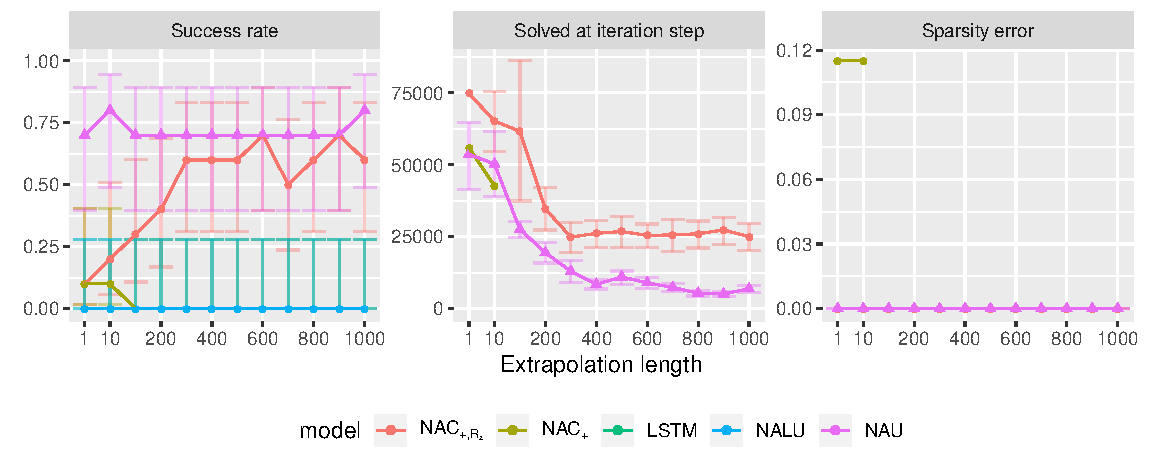
\includegraphics[width=\linewidth,trim={0 0.5cm 0 0},clip]{paper/results/sequential_mnist_sum_long.pdf}
\caption{Shows the ability of each model to learn the arithmetic operation of addition and backpropagate through the arithmetic layer in order to learn an image-to-scalar value for MNIST digits. The model is tested by extrapolating to larger sequence lengths than what it has been trained on. The NAU and $\mathrm{NAC}_{+,R_z}$ models use the $\mathrm{R}_z$ regularizer from section \ref{section:results:cumprod_mnist}.}
\label{fig:sequential-mnist-sum}
\end{figure}

\subsection{Sequential addtion without the \texorpdfstring{$\mathrm{R}_z$}{R\_z} regularizer}
\label{sec:appendix:sequential-mnist-sum:ablation}

As an ablation study of the $\mathrm{R}_z$ regularizer, figure \ref{fig:sequential-mnist-sum-ablation} shows the NAU model without the $\mathrm{R}_z$ regularizer. Removing the regularizer causes a reduction in the success-rate. The reduction is likely larger, as compared to sequential multiplication, because the sequence length used for training is longer. The loss function is most sensitive to the 10th output in the sequence, as this has the largest scale. This causes some of the model instances to just learn the mean, which becomes passable for very long sequences, which is why the success-rate increases for longer sequences. However, this is not a valid solution. A well-behavior model should be successful independent of the sequence length.

\begin{figure}[h]
\centering
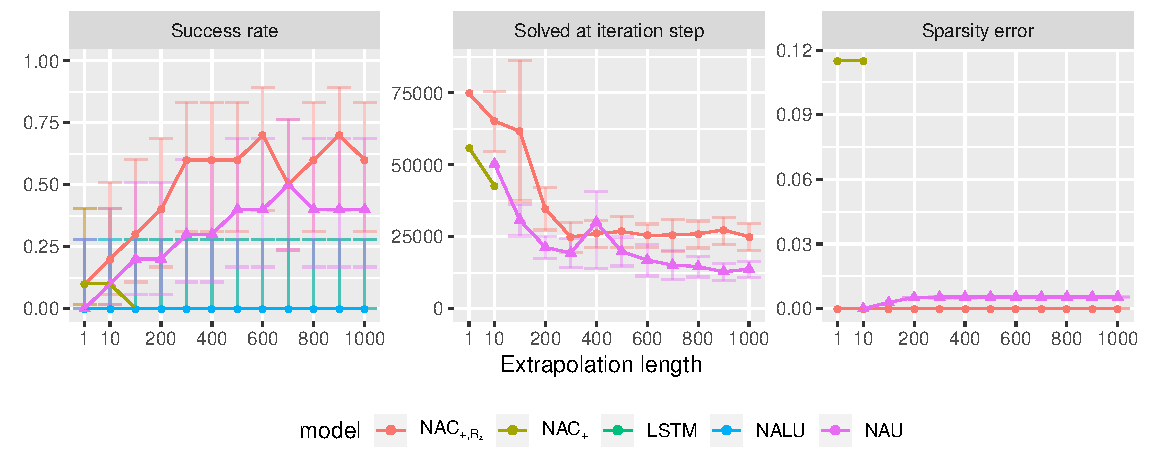
\includegraphics[width=\linewidth,trim={0 0.5cm 0 0},clip]{paper/results/sequential_mnist_sum_long_ablation.pdf}
\caption{Same as figure \ref{fig:sequential-mnist-sum}, but where the NAU model do not use the $\mathrm{R}_z$ regularizer.} 
\label{fig:sequential-mnist-sum-ablation}
\end{figure}

\subsection{Sequential multiplication without the \texorpdfstring{$\mathrm{R}_z$}{R\_z} regularizer}
\label{sec:appendix:sequential-mnist:ablation}

As an ablation study of the $\mathrm{R}_z$ regularizer figure \ref{fig:sequential-mnist-prod-ablation} shows the NMU and $\mathrm{NAC}_{\bullet,\mathrm{NMU}}$ models without the $\mathrm{R}_z$ regularizer. The success-rate is somewhat similar to figure \ref{fig:sequential-mnist-prod-results}. However, as seen in the ``sparsity error'' plot, the solution is quite different.

\begin{figure}[h]
\centering
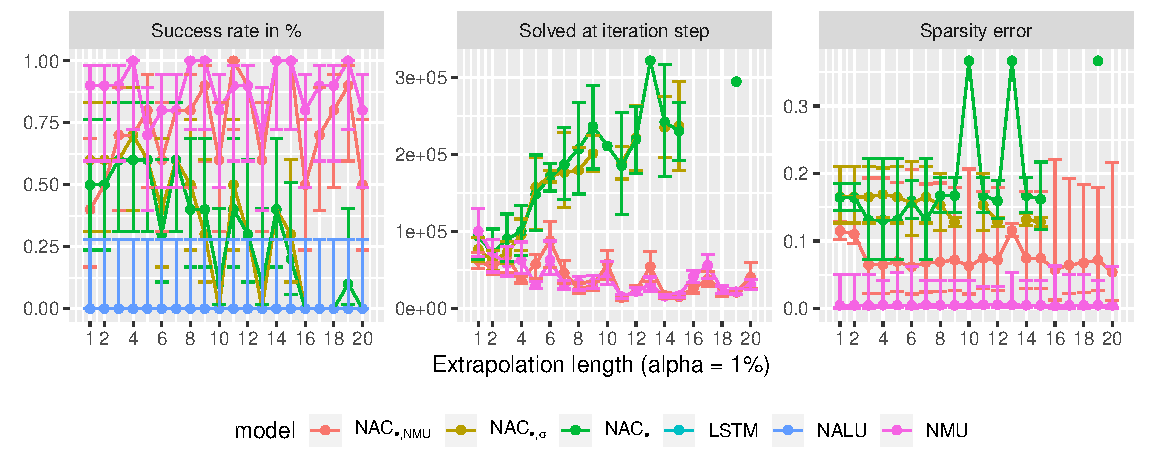
\includegraphics[width=\linewidth,trim={0 0.5cm 0 0},clip]{results/sequential_mnist_prod_long_ablation.pdf}
\caption{Shows the ability of each model to learn the arithmetic operation of addition and backpropagate through the arithmetic layer in order to learn an image-to-scalar value for MNIST digits. The model is tested by extrapolating to larger sequence lengths than what it has been trained on. The NMU and $\mathrm{NAC}_{\bullet,\mathrm{NMU}}$ models do not use the $\mathrm{R}_z$ regularizer.} 
\label{fig:sequential-mnist-prod-ablation}
\end{figure}
\clearpage
%
\section{Additional notes}

\subsection{Language to Number Translation Tasks}
\label{sec:appendix:lanauge-to-number}

In the NALU paper, they include a ``Language to Number Translation Tasks'' that appears to perform multiplication, by applying a recurrent NALU. However, after contracting the authors this turns out not to be the case.

\begin{itemize}
\item Question: In 4.3, how big is the embedding layer output dimensionality?\\ Answer: From memory - i think it was 256.
\item Question: In 4.3, how big is the LSTM layer output dimensionality?\\ Answer: From memory - I think it was 10 (small)
\item Question: In 4.3, what output and input activation does the LSTM layer have, tanh? \\ Answer: It uses the standard LSTM construction - default in Tensorflow.
\item Question: In 4.3, is the Linear/NAC/NALU layer only used for the final element in the sequence? See diagram.\\ Answer: Correct.
\end{itemize}

\begin{figure}[h]
\centering
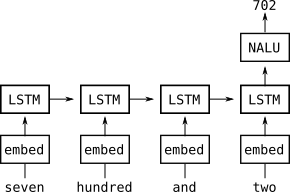
\includegraphics[scale=0.5]{graphics/language-to-numbers.png}
\caption{Diagram included in the email.} 
\end{figure}

Based on these answers, we don't believe ``Language to Number Translation Tasks'' tests multiplication in any meaningful way. There is nothing inherently wrong in that, as \citet{trask-nalu} don't state this explicitly either, we just wish to clarify this.

Our reasoning is that, an embedding of 256, is more than enough to fully describe every single token, keep in mind there are only 29 tokens in total. As such there is no reason why an LSTM layer wouldn't be able to solve this on its own (a simplified LSTM solving this task is seen in \eqref{eq:langauge-to-numbers-lstm}). Although, due to the non-linear activations, that are undesired in this case, the LSTM would need to downscale the values 0-1000 to be in the linear range of $\tanh(\cdot)$, and there would need to be final layer that upscales to 0-1000. We believe that the NALU layer serves this purpose and thus does not have any value in terms of arithmetics.

\begin{equation}
\begin{aligned}
h_t &= &h_{t-1}\ \cdot\ &f_t &&+ &\tilde{h}_{t}\ \ \cdot\ &i_t \\
h_t &= &\begin{bmatrix}
 h_{t-1} \\
 0 \\
 0
\end{bmatrix}^T &\left(I(x_t = \texttt{100})\begin{bmatrix}100 \\ 1 \\ 1\end{bmatrix}\right)\ &&+ &\begin{bmatrix}
 0 \\
 h_{t-1} \\
 x_t
\end{bmatrix}^T &\left(I(x_t \not= \texttt{100})\begin{bmatrix}100 \\ 1 \\ 1\end{bmatrix}\right)
\end{aligned}
\label{eq:langauge-to-numbers-lstm}
\end{equation}

%\clearpage

\end{document}